\section{E-R diagrams}
\subsection{Visio ER diagram}
\begin{figure}[h!]
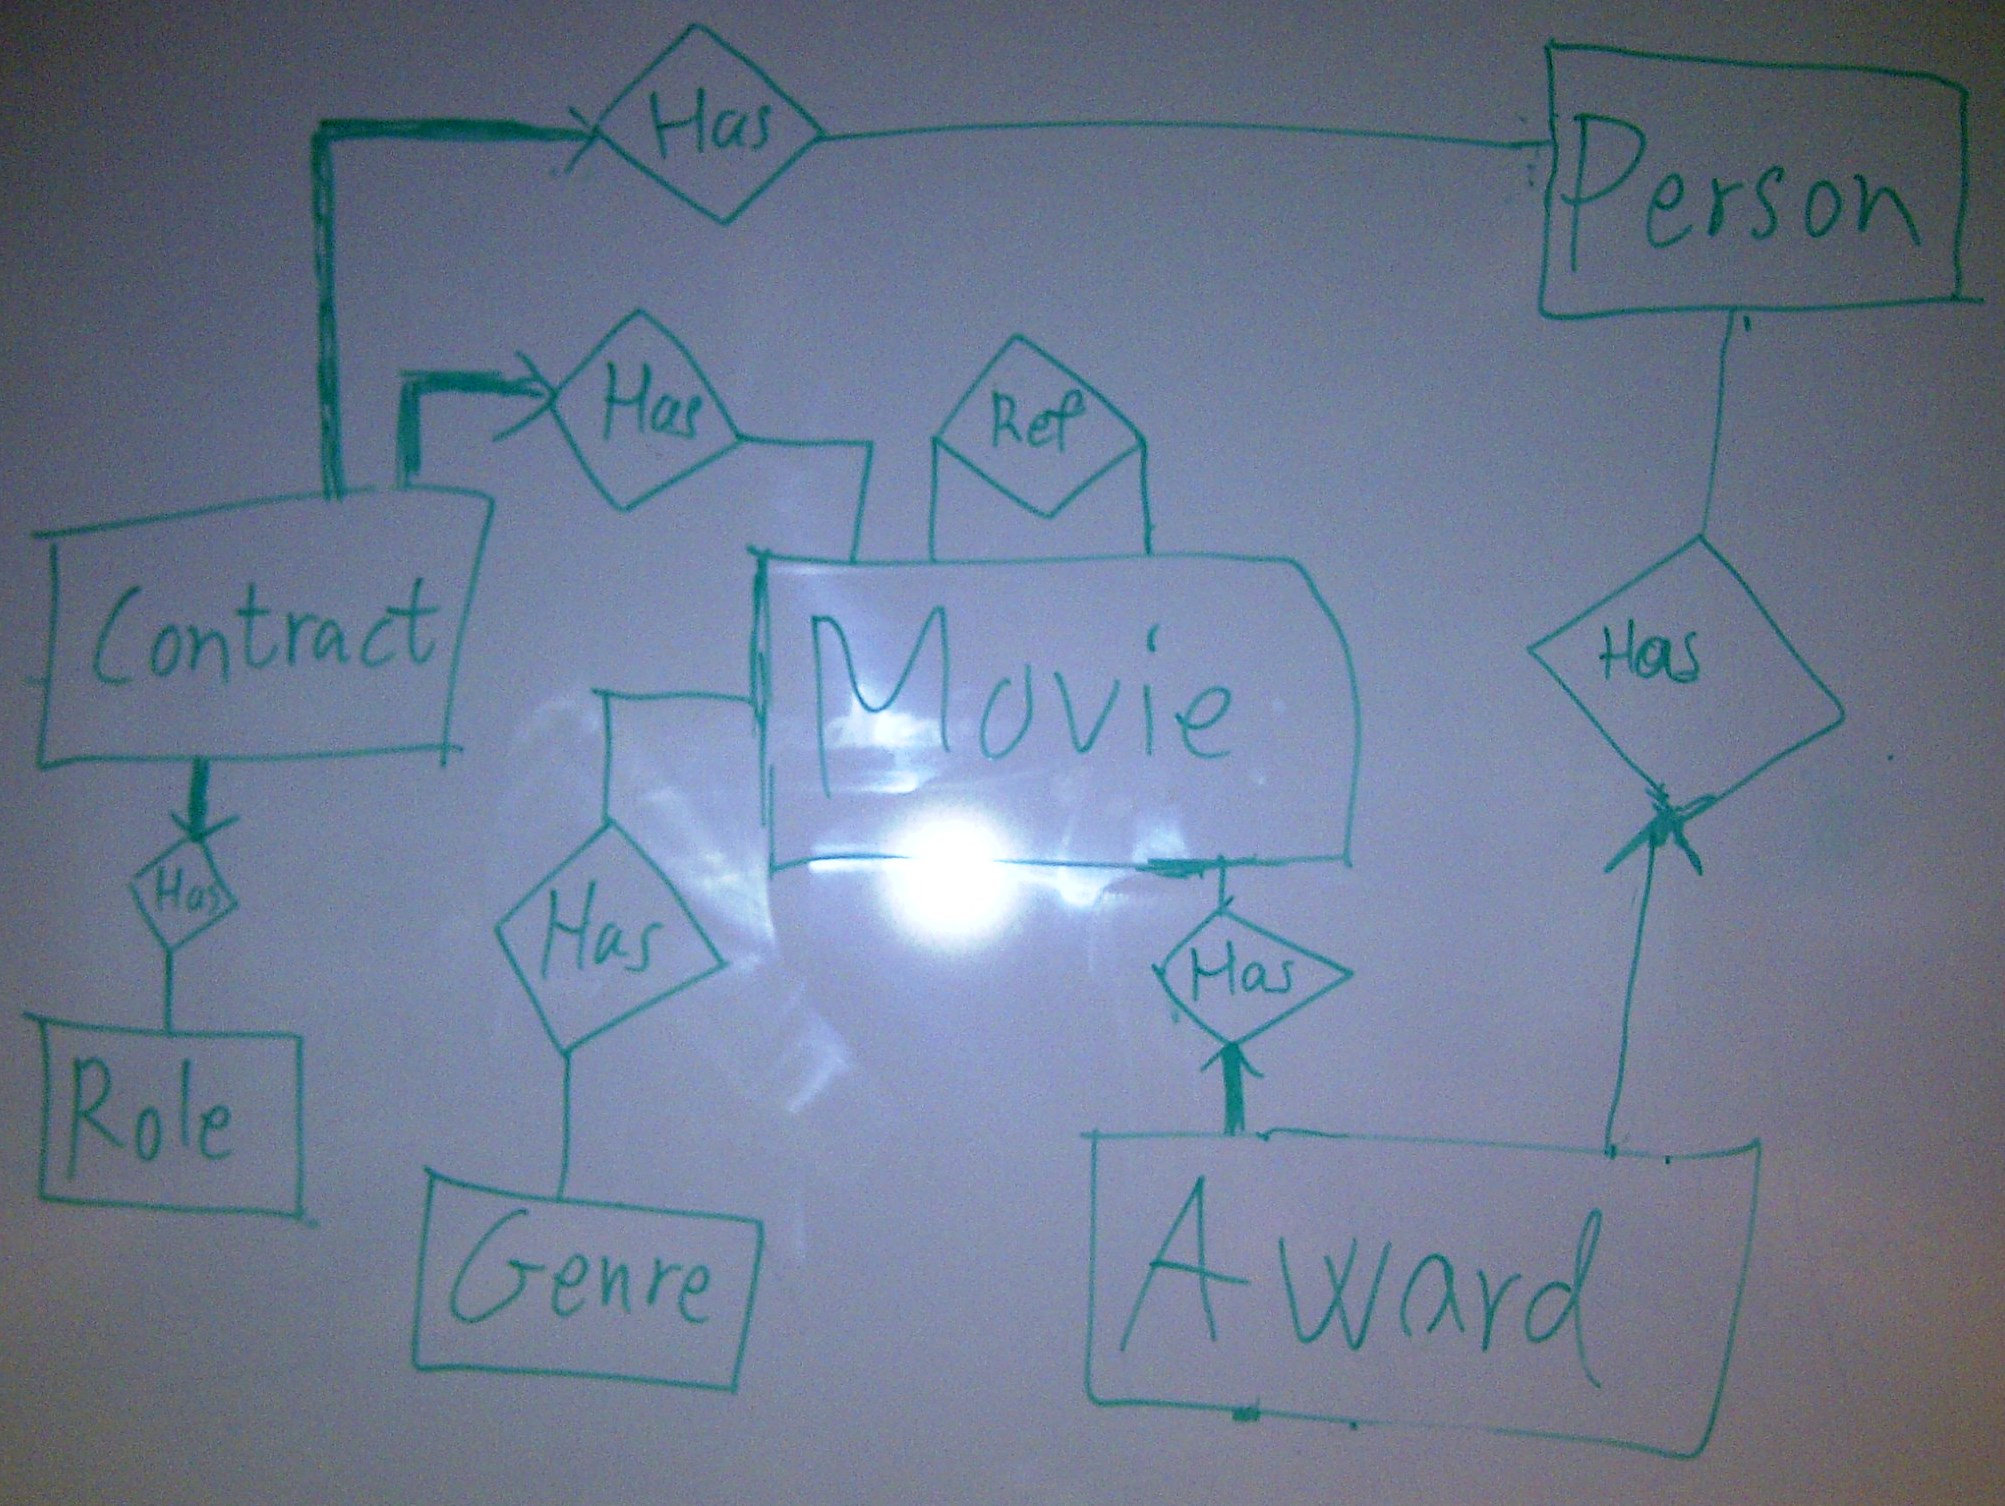
\includegraphics[width=\textwidth,natwidth=825,natheight=699]{illustrations/ER.jpg}
  \caption{Visio ER diagram}
\end{figure}
\subsection{Workbench RG diagram}
\begin{figure}[h!]
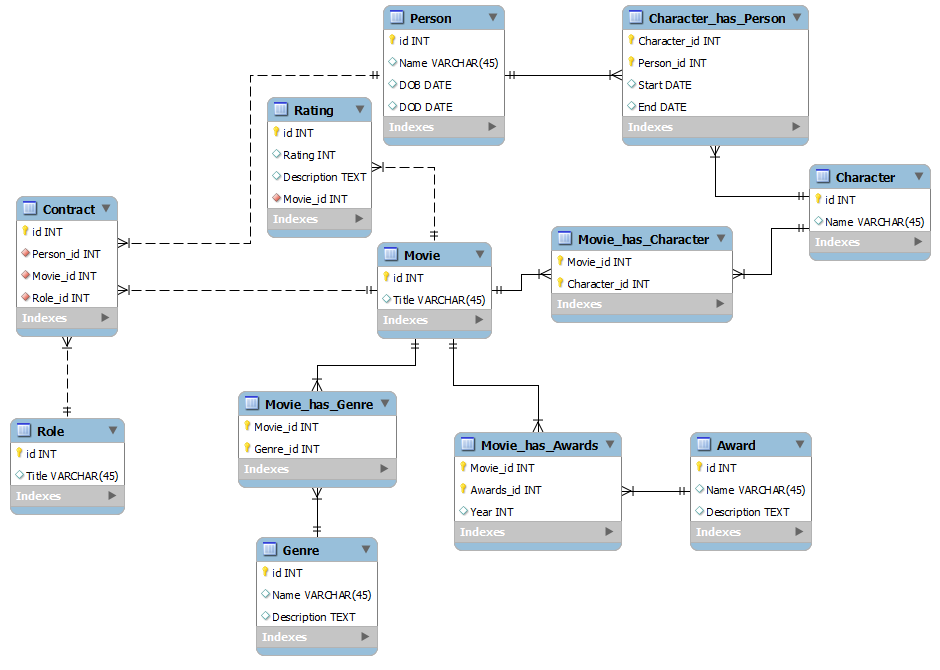
\includegraphics[width=\textwidth,natwidth=940,natheight=670]{illustrations/RG.png}
  \caption{New Workbench RG diagram}
\end{figure}
\newpage
\section{Changes since hand-in 1}
We have changed our model since our first hand-in. In our previous model an actor was unable to receive an award.
Our next order of business was filling our database with information from the given IMDB database. It quickly became apparent that our model lacked a few columns and that our model contained columns for which there is no data in the IMDB database.
Our new model is show on the diagram on the previous page. Following this is our old model:
\begin{figure}[h!]
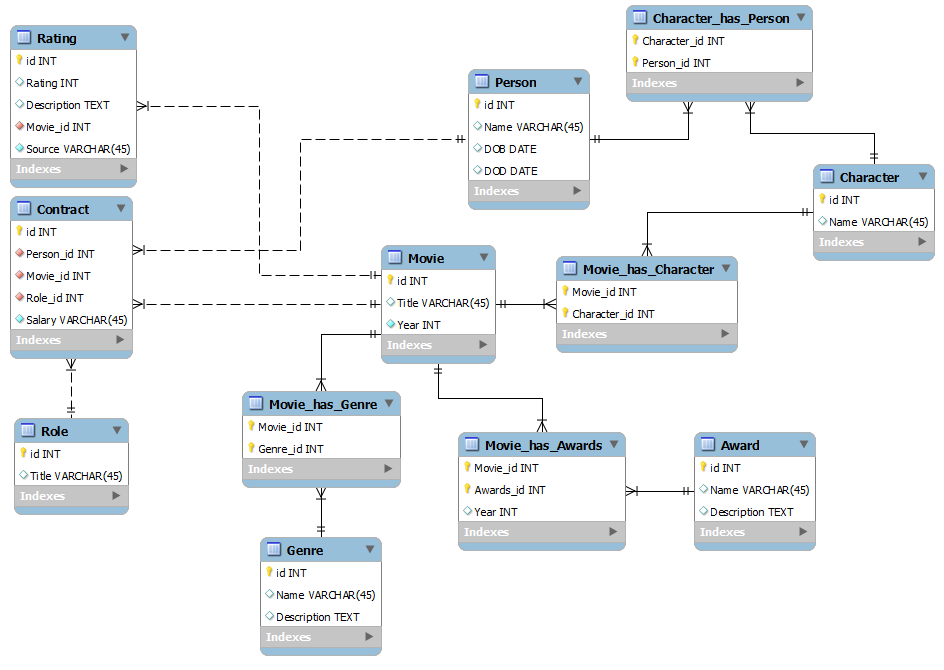
\includegraphics[width=\textwidth,natwidth=940,natheight=670]{illustrations/OldRG.png}
  \caption{Old Workbench RG diagram}
\end{figure}
\newpage
